\documentclass[10pt, twocolumn]{article}

%math
\usepackage{amsmath}
\usepackage{amssymb}
\usepackage{mathtools}
%logic
\usepackage{pgffor}
\usepackage{ifthen}
%science
\usepackage{siunitx}
\usepackage[version=4]{mhchem}
%language
\usepackage[english]{babel}
%formatting
\usepackage[a4paper, portrait, margin=1in]{geometry}
\usepackage{cuted}
\usepackage[small]{titlesec}
\usepackage[hidelinks]{hyperref}
\usepackage{parskip}
%images and plots
\usepackage{graphicx}
\usepackage[justification=centering]{caption}
\usepackage{subcaption}
\usepackage{float}
\usepackage{pgf}
\usepackage{import}
\usepackage{jsonparse}
%tables
\usepackage{booktabs}
\usepackage{makecell}
%citation, quatation and lists
\usepackage[style=numeric,maxcitenames=2,sorting=none,doi=false,
url=false,isbn=false,eprint=false]{biblatex}
\usepackage[noabbrev,nameinlink]{cleveref}
\usepackage{csquotes}
\usepackage[nottoc]{tocbibind}
\usepackage{acro}


%setup plugins
\addbibresource{literature.bib}

\captionsetup{justification=centering}
\hypersetup{colorlinks=true,linkcolor=blue}


\DeclareSIUnit\angstrom{\text {Å}}
\DeclareSIUnit\bar{bar}
\sisetup{
	range-phrase = { to }
}

% Custom \citeauthoryear command with hyperref -> Rost et al. (2019) 
\DeclareCiteCommand{\citeauthoryear}
{\boolfalse{citetracker}%
\boolfalse{pagetracker}%
\usebibmacro{prenote}}
{\ifciteindex
{\indexnames{labelname}\indexfield{year}}
{}%
\printtext[bibhyperref]{%
    \printnames{labelname}%
    \setunit{\addspace}%
    \printtext{(}%
    \printfield{year}%
    \printtext{)}}}
{\multicitedelim}
{\usebibmacro{postnote}}

%  setup custom commands
\newcommand{\imcite}[2][]{From \cite[#1]{#2}.}
\newcommand{\imcitetwo}[2][]{Based on \cite[#1]{#2}.}
\newcommand{\integral}[4]{\int_{#1}^{#2} #3 \mathrm{d} #4}
\newcommand{\derivative}[2]{\frac{\mathrm{d}}{\mathrm{d} #1} #2}

%import json
\JSONParseFromFile{\tasktwo}{../plots/task_2_data.json}
\JSONParseValue[store in = \taskTwoSlope]{\tasktwo}{concentration_m}
\JSONParseValue[store in = \taskTwoEnergy]{\tasktwo}{donor_energy}
\JSONParseValue[store in = \taskTwoSlopeOne]{\tasktwo}{mu_m1}
\JSONParseValue[store in = \taskTwoSlopeTwo]{\tasktwo}{mu_m2}
\JSONParseValue[store in = \taskTwoSlopeThree]{\tasktwo}{mu_m3}


% Document
\begin{document}
\pagenumbering{arabic}
\begin{strip}
	\begin{centering}
	\huge Semiconductor Physics Laboratory \RN{1}\\
	\LARGE A2: Scanning electron microscopy \\
	\vspace{0.35cm}
	\normalsize Simon Legtenborg, 3773994 \\ 
	\normalsize Experiment conducted on 22.11.2024 \\
	\vspace{1cm}
\end{centering}

\end{strip}
Die Breite einer Spalte beträgt: \the\columnwidth
\paragraph{Abstract}
This lab report explores various applications of a scanning electron
microscope.
Using secondary electron detection, the topography of an unknown
semiconductor sample is analyzed.
Additionally, material characteristics are determined through
X-ray emission and backscattered electrons.

\section{Free Carrier Statistics}
In order to draw conclusions about material properties by analyzing
the temperature dependence of the charge carrier density,
free carrier statistics and especially the influence of doping shall be
discussed.
\subsection{Charge Carrier Density}
The number of electrons per volume in the conduction band $n$ is
determined by the following expression:
\begin{equation}
	n=\int _{E_{\mathrm{C}}}^{\infty} D_{\mathrm{e}}(E)
	f_{\mathrm{e}}(E)\, \mathrm{d}E.
	\label{eq:n_int}
\end{equation}
In this equation, $E_{\mathrm{C}}$ represents the minimum energy level of
the conduction band. The function $D_{\mathrm{e}}(E)$ describes
the density of electronic states at a given energy $E$, while
$f_{\mathrm{e}}(E)$ is the statistical distribution function.
For electrons, this function is the Fermi-Dirac distribution that can be
defined with $E_\mathrm{f}$ as the Fermi-energy, $\mathrm{k}$ as the
Boltzmann constant and $T$ as temperature:
\begin{equation}
	f_{\mathrm{e}}(E)
	=\frac{1}{\exp((E-E_{\mathrm{F}})/(\mathrm{k}T))+1}.
\end{equation}
In order to solve the integral in \cref{eq:n_int}, a functional
expression for the density of states is required.
A suitable approximation that utilizes the effective electron mass
$m^*_\mathrm{e}$ are
parabolic band edges which originates from the free-electron gas:
\begin{equation}
	D(E)=\frac{1}{2\pi^2}
	\left( \frac{2m^*_\mathrm{e}}{\hbar^2} \right)^{3 / 2} \sqrt{E}.
	\label{eq:para_band_edges}
\end{equation}
By substituting \cref{eq:para_band_edges} into \cref{eq:n_int} and applying
the transformations $\eta=E_\mathrm{F}-E_\mathrm{C}$,
$x = (E-E_\mathrm{C}) / (\mathrm{k} T)$, the integral can be brought into
the following form:
\begin{align}
	n            & = N_\mathrm{c} \frac{2}{\sqrt{\pi}}
	\int_{0}^{\infty} \frac{\sqrt{ x }}{1+\exp(x-\eta / (\mathrm{k}T))} \,
	\mathrm{d}x \label{eq:n_int_2},                                        \\
	N_\mathrm{c} & = 2 \left( \frac{2 \pi m^*_\mathrm{e} \mathrm{k}T}{h^2}
	\right)^{3 / 2}.
\end{align}
\Cref{eq:n_int_2} represents a form of the Fermi-Dirac integral
$F_{1 /2}(\eta  / (\mathrm{k}T))$.
For $0 \gg \eta$,
this function can be approximated by $F_{1 /2}(\eta  / (\mathrm{k}T))
	\simeq \exp(\eta /(\mathrm{k}T))$.
Semiconductors that fulfill this requirement all called degenerate.
With that approximation, the free carrier density can be expressed as
a function of the Fermi-energy:
\begin{equation}
	n	= { N_{\mathrm{C}} }\exp\left( \frac{E_{\mathrm{F}}
		-E_{\mathrm{C}}}{\mathrm{k_B}T} \right).
	\label{eq:n}
\end{equation}
The same procedure can be applied in an analogous way for holes instead of
electrons.
Let $p$ be the number of holes per volume in the valence band,
one finds with similar assumptions:
\begin{align}
	p            & = N_\mathrm{V} \exp
	\left( - \frac{E_{\mathrm{F}}-E_{\mathrm{V}}}{\mathrm{k}T} \right)^{3 / 2}
	\label{eq:p},                                        \\
	N_\mathrm{V} & = 2 \left( \frac{2 \pi m^*_\mathrm{h}
		\mathrm{k}T}{h^2} \right).
\end{align}

\subsection{Intrinsic Conduction}
For an ideally pure semiconductor, only valence-band electrons
can exite into the conduction band.
This leads to the following charge neutrality condition:
\begin{equation}
	n = p.
\end{equation}
With this additional constraint, a formula for the free
carrier concentration can be found that only depends on the
band gap $E_\mathrm{g} = E_\mathrm{C} - E_\mathrm{V}$ by
substituting \cref{eq:n} and \cref{eq:p}
into the root below:
\begin{align}
	p & = n = \sqrt{n^2} = \sqrt{n \cdot p} \notag \\
	  & =\sqrt{ N_{\mathrm{V}}N_{\mathrm{C}} }
	\exp\left( -\frac{E_{\mathrm{g}}}{2\mathrm{k}T} \right).
\end{align}

\subsection{Donors and Acceptors}
\begin{figure*}
	\centering
	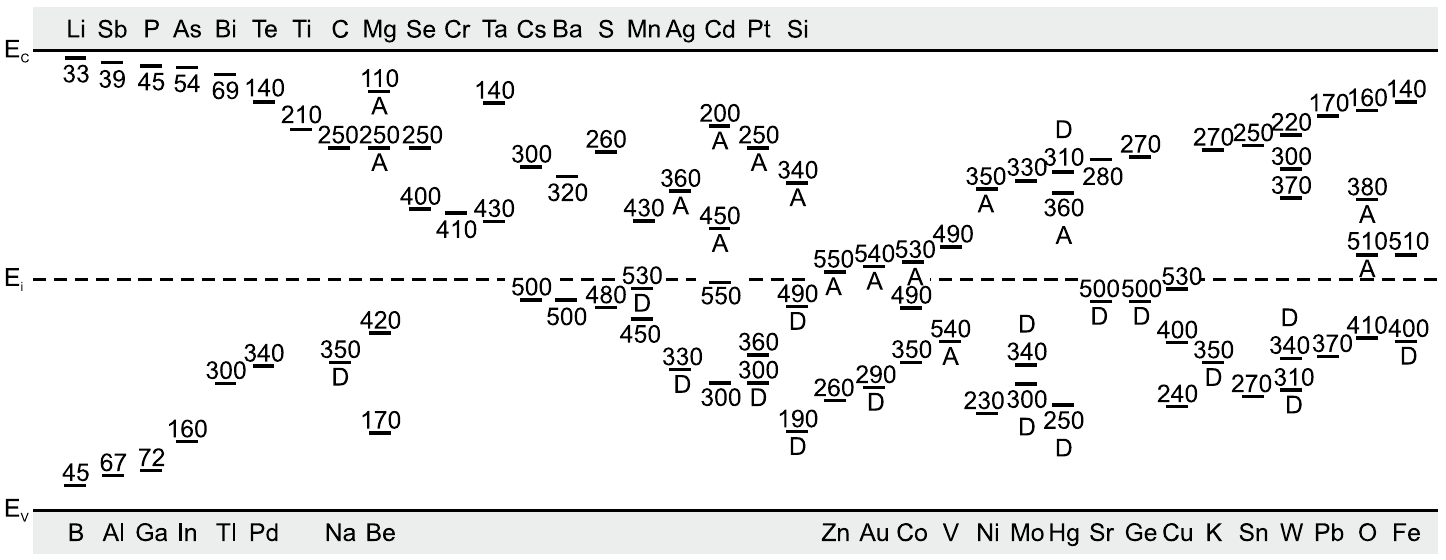
\includegraphics[width=0.6\linewidth]{../assets/energy_level.png}
	\caption{Energetic position of various donors and acceptors
		for silicon. \imcite{grundmann}}
	\label{fig:energy_level}
\end{figure*}

The conductivity of a semiconductor can be altered using
point defects.
This process is called doping.
If the conductivity is determined by holes, the material is
called p-type.
If the conductivity is determined by electrons, the material
is called n-type.

\paragraph{Donors} are point defect atoms that are incorporated into the crystal
lattice and dispose an additional electron after satisfying all
lattice bonds.
For group-$\mathrm{IV}$ semiconductors, group-$\mathrm{V}$ elements
are donors.
This extra electron is bound to the atom via Coulomb interaction,
which is a result of the higher charge of the donor's core.
The energy level of this electron can be estimated by assuming
energetically rescaled hydrogen orbitals.
This rescaling originates from the effective electron mass and
the screening of the coulomb interaction by the dielectric constant
of the material.
The absolute energetic position of the bound electron is
$E_{\mathrm{D}}=E_{\mathrm{C}}-E_{\mathrm{D}}^{b}$ with
\begin{equation}
	E_{\mathrm{D}}^{b}=
	\frac{1}{\epsilon_{\mathrm{r}}^{2}}
	\frac{m_{\mathrm{e}}^{*} e^{4}}{2(4\pi\epsilon_{0}\hbar)^{2}}.
\end{equation}
Energetic positions of various donors are displayed in
\cref{fig:energy_level}.
Similar to intrinsic conduction, the additional electrons have a
finite probability to shift into the conduction band
(they donate an electron) and
can therefore be used for n-type doping.
The probability for an electron to occupy the bound state $f^0$
(where '$0$' indicates that the donor is neutral) can be expressed
by the Fermi-Dirac distribution.
The probability for an electron to not occupy the bound state $f^+$
(where '$+$' indicates that the donor is ionized) can also be
determined:
\begin{align}
	f_{0} & =\frac{1}{1+\frac{g_{+}}{g_{0}}\exp\left(
	\frac{E_{\mathrm{D}}-E_{\mathrm{F}}}{\mathrm{k}T}\right)},  \\
	\label{eq:fplus}
	f_{+} & =(1-f_{0})=\frac{1}{1+\frac{g_{0}}{g_{+}}\exp\left(
		\frac{E_{\mathrm{F}}-E_{\mathrm{D}}}{\mathrm{k}T} \right)}.
\end{align}
Note that the degeneracy of the states impact the distribution.
A neutral donor has a degeneracy of $g^0=2$, since the bound
electron can take two spin states, the degeneracy of the
ionized donor is simply $g^+=1$.

Either the electron occupies the bound state or it shifts into the
conduction band.
Let $N_\mathrm{d}$ be the donor concentration, $N_\mathrm{d}^0$ the
number of neutral donors and $N_\mathrm{d}^+$ the number of ionized donors.
One finds the following relations:
\begin{align}
	N_{\mathrm{D}}     & =N_{\mathrm{D}}^{+}+N_{\mathrm{D}}^{0},        \\
	N_{\mathrm{D}}^{0} & \simeq N_{\mathrm{D}}f_0                             \\
	\label{eq:ndplus}
	N_{\mathrm{D}}^{+} & \simeq N_{\mathrm{D}}(1-f_{0}) =N_{\mathrm{D}}f_{+}.
\end{align}

\paragraph{Acceptors} are point defect atoms that are incorporated
into the crystal
lattice and lack one binding electron.
They are able to borrow (accept) an electron from the valence band.
For group-$\mathrm{IV}$ semiconductor, elements from group-$\mathrm{III}$
can be used as acceptors.
The energetic considerations are similar to those of donors.
The energy level of an electron that is bound to the acceptor can be
expressed
$E_{\mathrm{A}}=E_{\mathrm{V}}+E_{\mathrm{A}}^{b}$,
where $E_\mathrm{A}^b$ can be represented by rescaled
hydrogen orbitals.

These levels are also displayed in \cref{fig:energy_level}.
The acceptor concentration $N_\mathrm{A}$ can be separated into
the number per volume of ionized acceptors $N_\mathrm{A}^-$ and neutral
acceptors $N_\mathrm{A}^0$, such that the relation
$N_{\mathrm{A}}=N_{\mathrm{A}}^{0}+N_{\mathrm{A}}^{-}$ holds.
Again the probability of finding an electron bound to an acceptor $f$ is
equal to the probability of a hole shifted from the acceptor to the
valence band and can be modelled by a Fermi-Dirac-distribution:
\begin{equation}
	f = \frac{1}{1+\hat{g}_{\mathrm{A}}\exp\left( -
	\frac{E_{\mathrm{F}}-E_{\mathrm{A}}}{\mathrm{k}T} \right)}.
\end{equation}
In this case, the ratio of the acceptor state degeneracies
$\hat{g}_\mathrm{A}$ are nontrivial and need to be considered in detail.

\subsection{Charge Neutrality Condition}
Since donors and acceptors offer additional electrons or holes, the charge neutrality 
condition needs to be modified:
\begin{equation}
	n = p -\sum_i N_{\mathrm{A}i}^- + \sum_j N_{\mathrm{D}j}^+.
	\label{eq:charge_neutrality}
\end{equation}
\Cref{eq:charge_neutrality} can be used to get an implicit functional dependence $f(n,T)$.
A simple example is a material that is doped by only one donator material.
By using \cref{eq:ndplus} and additionally assume sufficient low
temperatures, intrinsic conduction can be neglected and the charge
neutrality condition is reduced to $n = N_\mathrm{D}^+=N_\mathrm{D} f_+$.
Substituting \cref{eq:n} and \cref{eq:fplus} results in:
\begin{align}
	\notag
	n     & =\frac{N_{\mathrm{D}}}{1+\hat{g}
		\exp\left( \frac{E_{\mathrm{F}}-E_{\mathrm{C}}}{\mathrm{k}T} \right)
	\exp\left( \frac{E_{\mathrm{C}}-E_{\mathrm{D}}}{\mathrm{k}T} \right)}                   \\
	\notag
	      & =\frac{N_{\mathrm{D}}}{1+ \hat{g}n /N_{\mathrm{C}}\cdot
	\exp\left( \frac{E_{\mathrm{C}}-E_{\mathrm{D}}}{\mathrm{k}T} \right)}, \label{eq:n_quad} \\
	      & =\frac{N_{\mathrm{D}}}{1+n / n_{1}},                                             \\
	n_{1} & =	\frac{N_{\mathrm{C}}}{\hat{g}}
	\exp\left( -\frac{E_{\mathrm{D}}^{b}}{\mathrm{k}T} \right)
\end{align}
\Cref{eq:n_quad} is a quadratic equation in terms of $n$ and thus
analytically solvable.
This leads to an explicit temperature dependence that can be approximated
for low and high temperature. 
\begin{equation}
	\label{eq:n_T}
	n = \frac{2N_{\mathrm{D}}}{1+\left( 1+4\hat{g} \frac{N_{\mathrm{D}}}{N_{\mathrm{C}}}
	\exp\left( \frac{E_{\mathrm{D}}^{b}}{\mathrm{k}T} \right) \right)^{1/2}},
\end{equation}
\begin{align}
	\label{eq:n_T_approx_low}
	n & \simeq \sqrt{ \frac{N_{\mathrm{D}}N_{\mathrm{C}}}{\hat{g}} }
	\exp\left( \frac{-E_{\mathrm{D}}^{b}}{2 \mathrm{k}T} \right) & \mathrm{k}T\ll 
	E_{\mathrm{D}}^{b} \\
	\label{eq:n_T_approx_high}
	n & \simeq N_{\mathrm{D}} & \mathrm{k}T\gg E_{\mathrm{D}}^{b}
\end{align}

\begin{figure}
	\centering
	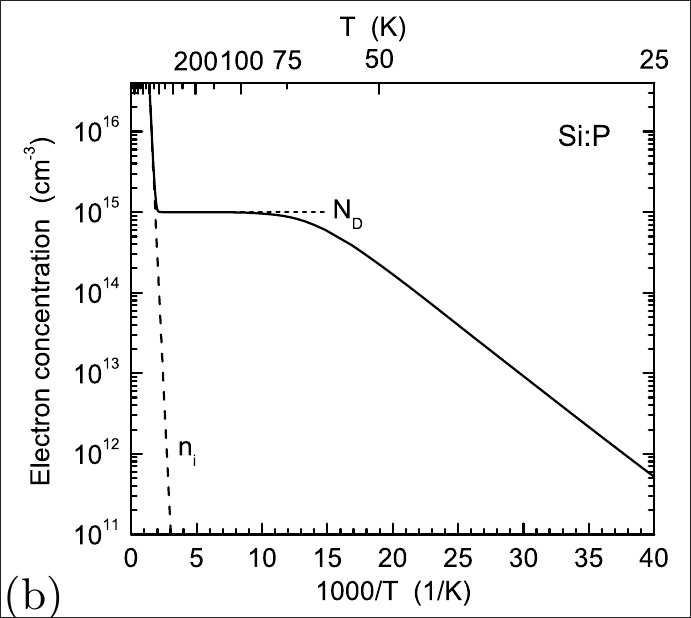
\includegraphics[width=0.75\linewidth]{../assets/charge_carrier_density_temperature.png}
	\caption{Charge carrier density as a function of temperature for 
	silicon doped with phosphor. \imcite{grundmann}}
	\label{fig:carrier_temperature}
\end{figure}
$n(T)$ is visualized in \cref{fig:carrier_temperature}.
Note that intrinsic conduction cannot be neglected for sufficient high
temperatures.
\section{Hall effect}
\begin{figure*}
	\centering
	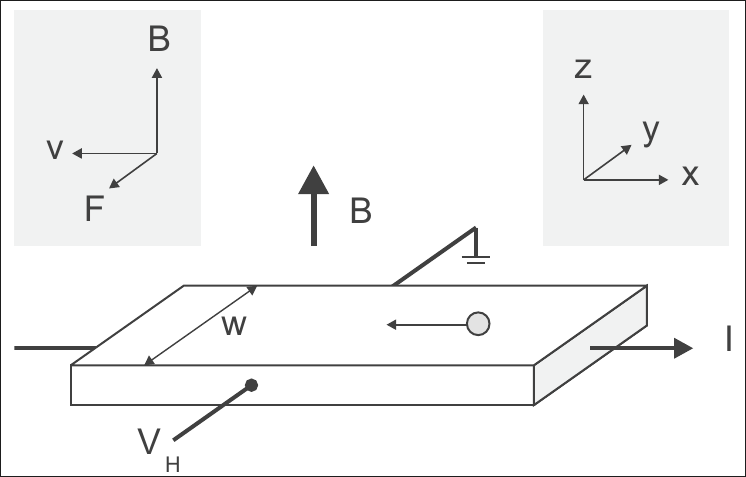
\includegraphics[width=0.8\linewidth]{../assets/hall_geometry.png}
	\caption{Schematic structure for Hall effect measurements.
		\imcite{grundmann}}
	\label{fig:hall}
\end{figure*}
The geometrical arrangement required for Hall effect measurements
is displayed in \cref{fig:hall}.
A magnetic field $\mathbf{B}=B \cdot \hat{z}$ penetrates
a semiconductor sample.
A current $\mathbf{j}$ is flowing along the $x$-direction inside the sample 
as a response to an external electric field $\mathbf{E}=E_x \cdot \hat{x}$.
Due to the magnetic force, the electrons are deflected and a current in
$y$-direction establishes until the resulting electric force in $y$-direction
fully compensates the magnetic force.
The system equilibrates for $j_y=0$.

To describe the system in detail for one majority charge carrier, one can use the 
equation of motion from relaxation time approximation:
\begin{equation}
	m^{*} \frac{\mathbf{v}}{\tau}=q(\mathbf{E}
	+\mathbf{v}\times \mathbf{B}).
\end{equation}
In this equation, $m^{*}$ is the effective mass of the charge carrier, $\mathbf{v}$ the
average electron velocity and $\tau$ the relaxation time constant.
With $\mathbf{j}=nq\mathbf{v}$ and the resistivity tensor $\hat{\rho}$, 
this vector equation can be brought into a linear transformation of the form
$\mathbf{E}=\hat{\rho}\mathbf{j}$ or more explicit:
\begin{equation}
	\label{eq:mej}
	\begin{pmatrix}
		E_{x} \\
		E_{y} \\
		E_{z}
	\end{pmatrix}
	=
	\begin{pmatrix}
		\frac{m^{*}}{\tau nq^{2}} & - \frac{B_{z}}{nq}        & 0                         \\
		\frac{B_{z}}{nq}          & \frac{m^{*}}{\tau nq^{2}} & 0                         \\
		0                         & 0                         & \frac{m^{*}}{\tau nq^{2}}
	\end{pmatrix}
	\begin{pmatrix}
		j_{x} \\
		j_{y} \\
		j_{z}
	\end{pmatrix}.
\end{equation}
The system equilibrates for $\mathbf{j} = j_x \cdot \hat{x}$ and with \cref{eq:mej}, the following
relationship holds true: $E_{y} = B_{z} / (nq) j_{x} = R_{\mathrm{H}}B_{z}j_{x}$.
This leads to an expression for the carrier density $n$ using directly measurable quantities.
\begin{align}
	R_{\mathrm{H}}&=\frac{1}{nq}=\frac{E_{y}}{j_{x}B_{z}}\\
	n&=\frac{j_{x}B_{z}}{E_{y}q}
\end{align}

Now we want to find an expression for the mobility.
\begin{equation}
	\begin{pmatrix}
		E_{x} \\
		E_{y} \\
		E_{z}
	\end{pmatrix}
	=\begin{pmatrix}
		\mu_\mathrm{H}^{-1} & -B_{z}              & 0                   \\
		B_{z}               & \mu_\mathrm{H}^{-1} & 0                   \\
		0                   & 0                   & \mu_\mathrm{H}^{-1}
	\end{pmatrix}
	\begin{pmatrix}
		v_{x} \\
		v_{y} \\
		v_{z}
	\end{pmatrix}
\end{equation}
The hall mobility in this equation is defined as $\mu_{\mathrm{H}}=\frac{q\tau}{m^{*}}$.
To see why this is useful, first, think of the limit $B_{z}\to 0$.
Then, electric field and velocity indeed follow the relation $\mathbf{v}=\mu_{\mathrm{h}}\mathbf{E}$.
Second with $\mathbf{v}=\mu_{\mathrm{h}}\mathbf{E}$ one can easily see that
$v_{x} = \mu_{\mathrm{H}}E_{x}$ and $E_{y}=B_{z}v_{x}=B_{z}\mu_{\mathrm{H}}E_{x}$.
Therefore we find the following equation for $\mu_\mathrm{H}$:
\begin{equation}
	\mu_{\mathrm{H}}=\frac{E_{y}}{B_{z}E_{x}}
\end{equation}

\subsection{Van der Pauw Method}
The Van der Pauw Method is a measuremtn technique to measure the resistivity as well as the hall coefficient.
It is possible to measure samples with nearly arbitrary flat shapes and examine it's resistivity $\rho$, 
mobility $\mu_\mathrm{H}$ as well as it's sheet carrier density $n$. 

Only samples that met the subsequent conditions can be measured with the Van der Pauw method:
\begin{itemize}
	\item The contacts are at the circumference of the sample.
	\item The contacts are sufficiently small (compared to the sample size).
	\item The sample is homogeneous and isotropic cocerning doping as well as thickness.
	\item The surface of the sampele is singly connected, i.e., the sample does not have isolated holes.
\end{itemize}
To utilize the Van der Pauw method, four ohmic contacts need to be placed on the sample.
These contacts should be as small as possible and as close as possible to the samples periphery. 
All contacts and all wires should be constructed from the same material. 

After the ohmic contacts are places, the resistivity $\rho$ can be measured.
Each contact is labeled counterclockwise with a number from 1 to 4.
The current $I_{12}$ is then defined as the positive current injected into contact one and extracted from contact two.
The voltage $V_{34}$ is given by the potential difference between contact three and four as $V_{34}=V_4-V_3$. 
With these definitions, the resistivity can be calculated as $R_{12,34}=\frac{V_{34}}{I_{12}}$. 
Van der Pauw's theorem states that the resistivity can be calculated as 
$$
\begin{align}
\rho&=\frac{\pi d}{\ln(2)} \left( \frac{R_{12,34}+R_{23,41}}{2} \right)f
\left( \frac{R_{12,34}}{R_{23,41}} \right) \\
\label{eq:hall_resistivity}\\
\frac{R_{12,34}-R_{23,41}}{R_{12,34}+R_{23,41}}&=f \, \text{arccosh}\left( \frac{\exp(\ln(2 /f))}{2} \right)
\label{eq:hall_resistivity_f}
\end{align}
$$
where $d$ is the thickness of the sample and $f$ is a correction factor that satisfies \cref{eq:hall_resistivity_f}. 
The reciprocal theorem states that the resistances obey the relation $R_{12,34}=R_{34,12}$ and $R_{12,34}=R_{21,43}$.
Therefore, we can measure the resistivity with four different contact configurations to increase measurement accuracy.

Within the Van der Pauw configuration, it is also possible to determine the Hall coefficient $R_{\mathrm{H}}$ if 
one can establish a homogeneous magnetic field $\mathbf{B}=B_{0} \hat{z}$ perpendicular to the samples surface. 
The Hall coefficient can be calculated as
$$
R_{\mathrm{H}}=\frac{d}{IB_{z}} [U_{13}(B_{z}=0)-U_{13}(B_{z}=B_{0})].
\label{eq:hall_coefficient}
$$
The difference in  \cref{eq:hall_coefficient} accounts for the Hall voltage that originates from the earths magnetic field.




\section{Results and Discussion}
\subsection{Hall Effect Measurements at Room Temperature}
Measurements were performed on p-type silicon (\ce{p-Si}, $d=\qty{500}{\micro\meter}$), 
zinc oxide (\ce{ZnO}, $d=\qty{1}{\micro\meter}$), zinc tin oxide (\ce{ZTO}, 
$d=\qty{1.3}{\micro\meter}$) and copper iodide (\ce{CuI}, $d=\qty{0.339}{\micro\meter}$) 
thin film samples.
Using the Van der Pauw method, the resistivity, Hall carrier concentration and Hall 
coefficients were determined for each sample.

With four distinct sample contact configurations, four measurements were performed 
per sample. 
The resistivity $\rho$ was calculated using \cref{eq:hall_resistivity}, 
the Hall coefficient $R_{\mathrm{H}}$ using \cref{eq:hall_coefficient_van_der_pauw},
the carrier concentration $n$ using \cref{eq:hall_concentration} 
and the Hall mobility $\mu_{\mathrm{H}}$ using \cref{eq:hall_mobility}.
The results are averaged in \cref{tab:hall_results_detail}, 

An important observation is the varying sign of $R_{\mathrm{H}}$. 
Since the sign of the Hall coefficient is determined by the majority charge carrier
(positive for holes, negative for electrons), this indicates that holes are the majority
charge carrier for \ce{p-Si} and \ce{CuI}. 
Electrons are the majority charge carrier for \ce{ZnO} and \ce{ZTO}. 

\subsection{Temperature Dependent Hall Effect Measurements}
Temperature dependent Hall effect measurements for a bulk \ce{ZnO} sample 
were performed in the Temperature range from \qty{20}{\kelvin} to \qty{325}{\kelvin}.
Both the Hall mobility and Hall carrier concentration were determined for each 
temperature and are displayed in 
\cref{fig:zno_hall_effect_n,fig:zno_hall_effect_mu} respectively.

The graph of the Hall carrier concentration in \cref{fig:zno_hall_effect_n} shows a 
linear decrease with increasing inverse temperature. 
This observation can be explained using the low temperature approximation 
\cref{eq:n_T_approx_low}:

\begin{align}
	&n = \text{const.} \cdot T^{3/2} \exp\left( \frac{-E_{\mathrm{D}}^{b}}{2 \mathrm{k}T} \right) \\
	\ln(&n T^{-3/2}) = \ln(\text{const.}) - \frac{E_{\mathrm{D}}^{b}}{2 \mathrm{k}} \cdot \frac{1}{T} 
	\label{eq:n_T_approx_low_linear}
\end{align}

Using a linear fit, one obtains a slope of \qty{\taskTwoSlope}{\kelvin}.
With \cref{eq:n_T_approx_low_linear}, this slope can be used to determine the donor energy 
$E_{\mathrm{D}}^{b} = \qty{\taskTwoEnergy}{\milli \electronvolt}$.
For high temperatures, the carrier concentration saturates, since all donors are ionized.
By applying \cref{eq:n_T_approx_high}, the donor concentration can be estimated to be
$N_{\mathrm{D}} = \qty{\taskTwoND}{\per \meter\cubed}$.

The Hall mobility in \cref{fig:zno_hall_effect_mu} can be parted into three distinct 
regions.
For every region, the data follows a linear trend, that can be described using three 
linear fits.
The first region has a slope of \num{\taskTwoSlopeOne}, the second region has a slope of
\num{\taskTwoSlopeTwo} 
and the third region has a slope of \num{\taskTwoSlopeThree}.

In a $\log-\log$ plot, a linear function indicates a power law relationship, whereby the
slope of the line corresponds to the exponent of the power law. 
Since the mobility is determined by scattering processes, that have a characteristic 
temperature dependence, different scattering mechanisms can be identified. 
The first region, where $\mu_\mathrm{H} \propto T^{3 / 2}$, can be explained by 
ionized impurity scattering.
The second region, where $\mu_\mathrm{H} \propto T^{\taskTwoSlopeTwo} \simeq T^{-1/2}$, 
can be explained by piezoelectric potential scattering.
The third region, where $\mu_\mathrm{H} \propto T^{\taskTwoSlopeThree} 
\simeq T^{-3 / 2}$, can be explained by deformation potential scattering.

\begin{figure*}
	\centering
	\begin{subfigure}{0.48\textwidth}
		\centering
		\includegraphics{../plots/task_2_n.pdf}
		\caption{Hall carrier concentration of a bulk \ce{ZnO} sample as a function of temperature.}
		\label{fig:zno_hall_effect_n}
	\end{subfigure}
	\hfill
	\begin{subfigure}{0.48\textwidth}
		\centering
		\includegraphics{../plots/task_2_mu.pdf}
		\caption{Hall mobility of a bulk \ce{ZnO} sample as a function of temperature.}
		\label{fig:zno_hall_effect_mu}
	\end{subfigure}
	\caption{Temperature-dependent Hall effect measurements of a bulk \ce{ZnO} sample.}
	\label{fig:zno_hall_effect_combined}
\end{figure*}

\subsection{Interpretation of an Unusual Data Set}
Temperature dependent Hall effect measurements of a \ce{ZnO} thin film sample
were performed in the temperature range from \qty{20}{\kelvin} to \qty{325}{\kelvin}.
However, the dataset does not seem to match a single donor model, as the carrier 
concentration, see \cref{zno_hall_n} raises with falling temperature.
The uncorrected data is shown in \cref{zno_hall_n}, it does not show a linear trend. 

This could indicate that the sample is not a single donor system. 
However, \citeauthoryear{look} suggest, that the sample is a single donor system, 
but a two-layer Hall analysis needs to be performed to correct the data. 
Since \ce{ZnO} and sapphire have a large lattice mismatch, a highly dislocated region 
at the interface between thin film and substrate is generated during growth. 
This high-density region of stacking faults significantly affects the carrier 
concentration as well as the mobility as a function of temperature and does not
show a linear trend.

For a two-layer Hall analysis, we index the \ce{ZnO} thin film as '\num{1}' and the 
dislocated region at the interface as index '\num{2}'. 
Using \cref{eq:multilayer_sum_1,eq:multilayer_sum_2} we can find the following identities
\begin{align}
	\sigma_{\square}=e\mu_{\mathrm{H}1}n_{ \square 1}
	+e \mu_{\mathrm{H}2} n_{ \square 2} \\
	R_{\square} \sigma_{\square}^{2}=e \mu_{\mathrm{H} 1}^{2} n_{ \square 1} 
	+ e\mu_{\mathrm{H} 2}^{2} n_{ \square 2}
\end{align}
It is possible to find an analytical expression for 
$\mu_\mathrm{H}$ and $n$:
\begin{align}
	\mu_{\mathrm{H}}&=R_{\square} \sigma_{\square}
	=\frac{R_{\square} \sigma_{\square}^{2} /d}{\sigma_{\square} / d} \\
	&=\frac{\mu_{\mathrm{H}1}^{2}n_{1}
	+\mu_\mathrm{H2}^{2} n_{\square2} /d}{\mu_{\mathrm{H}1}n_{1}
	+\mu_{\mathrm{H}2}n_{\square{2}} /d} \\
	n_{}=\frac{n_{ \square}}{d}&=\frac{1}{eR_{\square}d}
	= \frac{\sigma^{2}_{\square}/ d^{2}}{eR_{\square}\sigma_{\square}^{2} / d}  \\
	&=\frac{(\mu_{\mathrm{H}1}n_{1}
	+\mu_{\mathrm{H}2}n_{\square2} /d)^{2}}{\mu_{\mathrm{H}1}^{2}n_{1}
	+\mu_{\mathrm{H}2}^{2} n_{ \square 2} /d}
\end{align}
Since the donor atoms freeze at low temperatures, the interface layer must be dominant 
in this region. 
Since the paper suggest that the layer's carrier concentration and mobility is 
temperature independent, we can approximate
$n_{}=n_{ \square 2} / d = \qty{\taskThreeInterfaceN}{\per\meter\cubed}$ 
and 
$\mu_{\mathrm{H}}=\mu_{\mathrm{H 2}} = \qty{\taskThreeInterfaceM}{\centi\meter\squared\per\volt\per\second}$
for $T \to \qty{0}{\kelvin}$. 

An expression for the corrected hall mobility $\mu_{\mathrm{H} 1}$ and  
hall carrier concentration $n_{1}$ can now 
be found:
\begin{align}
	\mu_{\mathrm{H} 1}=\frac{\mu_{\mathrm{H}}^{2} n_{}- \mu_{2} ^{2} 
	n_{ \square 2} /d}{\mu_{\mathrm{H}} n_{} - \mu_{2} n_{\square 2} / d} \\
	n_{1} = \frac{(\mu_{\mathrm{H}}n_{}-\mu_{2}n_{\square 2} 
	/ d)^{2}}{\mu_{\mathrm{H}}^{2}n_{}-\mu_{2}^{2} n_{\square 2} / d}	
\end{align}
The corrected carrier density is also displayed in \cref{zno_hall_n} and can
now be identified with the single-donor case.
Using linear regression, a slope of \num{\taskThreeSlope} and a corresponding donor 
energy of $\qty{\taskThreeEnergy}{\milli \electronvolt}$ can be determined.
The donor concentration can be estimated using \cref{eq:n_T_approx_high} to be
$N_{\mathrm{D}} = \qty{\taskThreeND}{\per\meter \cubed}$

The corrected mobility is displayed in \cref{zno_hall_mu} and shows a linear trend with a 
slope of \num{\taskThreeMobilityOne} for the first region and a slope of 
\num{\taskThreeMobilityThree} for the second region.
The log-log plot indicates a power law relationship, that can be explained by
deformation potential scattering since 
$\mu_\mathrm{H} \propto T^{\taskThreeMobilityThree} \simeq T^{-3/2}$.

\begin{figure*}
	\centering
	\begin{subfigure}[t]{0.48\textwidth}
		\centering
		\includegraphics{../plots/task_3_n.pdf}
		\caption{Corrected and uncorrected Hall carrier concentration of a \ce{ZnO} thin 
		film sample as a function of temperature.}
		\label{zno_hall_n}
	\end{subfigure}
	\hfill
	\begin{subfigure}[t]{0.48\textwidth}
		\centering
		\includegraphics{../plots/task_3_mu.pdf}
		\caption{Corrected and uncorrected Hall mobility of a \ce{ZnO} thin film sample as 
		a function of temperature.}
		\label{zno_hall_mu}
	\end{subfigure}
	\caption{Corrected and uncorrected Hall effect measurements of a \ce{ZnO} thin film sample.}
	\label{fig:zno_hall_effect_corrected}
\end{figure*}

\begin{table*}
\centering
\input{../plots/resistivity_hall.tex}
\caption{Hall effect quantities of p-Si, ZnO, ZTO and CUI thin film samples.}
\label{tab:hall_results_detail}
\end{table*}

\clearpage
\begin{strip}
	\printbibliography[heading=bibintoc]
	\listoffigures
	\listoftables
\end{strip}
$\phantom{=}$
\end{document}
